\newpage
%//------ Section 04 -------------------------------------------------------------------------------------------------
\chapter{Identification of V0 particles and cascades}
\label{chap:V0CascReconstruction}
%//-----------------------------------------------------------------------//

The \chap\ref{chap:ParticlePhysics} and \ref{chap:ALICE} have set the scene, it is time now for the main actors to come onto stage, that are the (multi-)strange baryons or more precisely, the \textit{hyperons}. These consist of any baryon containing at least one strange quark, but no heavier quarks such as charm, bottom (or top...). By describing their identification and the physics interests surrounding their reconstruction, this short chapter lays the foundations for the analyses performed throughout this thesis.\\

The first section, \Sec\ref{sec:StrangenessFeatures}, underlines the appealing features of strangeness and, particularly, (multi-)strange particles. The hyperons of interest in the present analyses are specified in the following section, \Sec\ref{sec:HyperonId}, as well as the motivations for this choice. This part also presents the principles for multi-strange baryon identification via topological reconstruction. Finally, in connection with \chap\ref{chap:ALICE}, this short chapter closes on what makes ALICE a unique experiment for studying strange hadrons.

\section{The appealing features of strangeness}
\label{sec:StrangenessFeatures}

\subsection{The strange quark with respect to the other flavours}

Similarly as for the charm, bottom and top quarks, there is no strangeness among the \emph{valence} quarks of the nucleons from the collision beams. At first sight, these only consist in up and down quarks. Admittedly, other quark flavours can still be found inside the sea of quarks and gluons, in amounts that rise as the momentum fraction carried by such initial partons gets smaller and smaller. However, those almost always do not take part in the collision processes\footnote{Gluon fusion processes dominate the collision picture from the very low momentum fraction~$x_{\rm B}$ up to $x_{\rm B} \approx 0.05$, that is, at mid-rapidity, to any outcome object originating from processes with energy transfer up to $Q = \sqrtS \cdot x_{\rm B} = 13~\tev \cdot 0.05 = 650~\gev$, meaning up to high energy scale.}. From this, there arises an interesting and straightforward aspect of strangeness: the vast majority of the strange quarks observed in the final state hadrons must have been produced in the processes that have occurred during the collision.\\

Another property regards the mass of the strange quark. One way of classifying quarks is based on whether they preserve (at least, approximatively) or break the chiral symmetry (\Sec\ref{subsubsec:chiralsymmetrybreaking}): the up and down quarks belongs to the first kind and makes part of the light flavour sector. Those breaking the chiral symmetry -- the charm, bottom and top quarks -- constitute the heavy flavour sector. For comparison, the \emph{bare} mass of the light flavour quarks sits in the \mmass-regime; the up quark at $2.16_{-0.26}^{+0.49}$ \mmass, the down quark at $4.67_{-0.17}^{+0.48}$ \mmass. In contrast, the one of the charm, bottom and top quarks lies in the \gmass-regime: $1.27 \pm 0.02$ \gmass, $4.18_{-0.02}^{+0.03}$ \gmass and $172.69 \pm 0.30$ \gmass respectively~\cite{particledatagroupReviewParticlePhysics2022}. From this perspective, the strange quark with its bare mass of $93.4_{-3.4}^{+8.6}$ \mmass holds a unique position: its lightweight makes it relatively inexpensive (in terms of energy) to produce; being still much heavier than the up and down quarks (by a factor between 20 and 50), this also qualifies it as non-ordinary matter. Thus viewed as both light and heavy, the strange quark gives access to an \emph{abundant} source of \emph{non-ordinary} matter and information about the collision dynamics.


\subsection{The specificity of strange hadrons}
\label{subsec:SpecStrangeHadrons}

Most of strange hadrons decays into charged particles in their dominant channel. In addition, they also have a relatively long lifetime, allowing them to fly over several centimeters before the decay. From these two elements stem the distinctive decay topology of strange particles known as V0 or cascade (\Sec\ref{subsec:V0CascDecays}), that can be used in their reconstruction by associating the different daughter tracks to reform the decay vertex (topological reconstruction, detailed later in \Sec\ref{subsec:TopoReco}) \cite{speltzCaracterisationEtatDense2006}. This characteristic turns out to be particularly interesting as it offers a good control of the background, thus providing a robust identification of strange hadrons over a wide momentum range, from low to high \pT.

Coupled to their abundant production, this feature offers the possibility for a continuous study of strange hadrons over different production regimes, involving soft, intermediate and hard processes such as multi-parton interactions, quark coalescence and jet fragmentation respectively. For that reason, strange particles represent prime-choice probes to investigate and thus improve our understanding on the evolution of the hadronisation mechanisms\footnote{To be exact, it is not the hadronisation mechanisms that evolves with the transverse momentum but rather their relative weight. For instance, quark coalescence happens mostly at intermediate \pT but it can still occur at high momentum, although with a different probability.} with momentum.

%Most of strange hadrons decays into charged particles in their dominant channel. In addition, they also have a relatively long lifetime, allowing them to fly over several centimeters before the decay. From these two elements stem the distinctive decay topology of strange particles known as V0 or cascade (\Sec\ref{subsec:V0CascDecays}), that can be used in their reconstruction by associating the different daughter tracks to reform the decay vertex (topological reconstruction, detailed later in \Sec\ref{subsec:TopoReco}) \cite{speltzCaracterisationEtatDense2006}. This characteristic turns out to be particularly interesting as the latter provides a robust identification of strange hadrons over a wide momentum range, from low to high \pT.
%
%Consequently, this offers the possibility for a continuous study of strange hadrons over different production regimes, involving soft, intermediate and hard processes such as multi-parton interactions, quark coalescence and jet fragmentation respectively. For that reason, strange particles represent prime-choice probes to investigate and thus improve our understanding on the evolution of the hadronisation mechanisms\footnote{To be exact, it is not the hadronisation mechanisms that evolves with the transverse momentum but rather their relative weight. For instance, quark coalescence happens mostly at intermediate \pT but it can still occur at high momentum, although with a different probability.} with momentum.

\section{The multi-strange baryon identification}
\label{sec:HyperonId}

Among all the strange hadrons, this work focuses on the strangest baryons, containing two or three strange quarks, the so-called multi-strange baryons. Excluding the associated resonances, this leaves five particles: three containing two strange quarks -- the \rmXiZero\ ($uss$), \rmXiM ($dss$) and \rmAxiP ($\bar{d}\bar{s}\bar{s}$) -- and two triple-strange hadrons namely the \rmOmegaM ($sss$) and \rmAomegaP ($\bar{s}\bar{s}\bar{s}$).

\begin{table}[h]
    \centering
    \begin{tabular}{b{2cm}@{\hspace{0.25cm}} b{2cm}@{\hspace{0.5cm}} b{2cm}@{\hspace{0.25cm}} b{2cm}@{\hspace{0.25cm}} b{3cm}@{\hspace{0.5cm}} b{1.5cm}@{\hspace{0.25cm}}}
    \noalign{\smallskip}\hline\noalign{\smallskip}
	Particle & Strangeness & Mass (\mmass) & Lifetime (\cm) & Dominant decay channel & B.R. \\
    \noalign{\smallskip}\hline \noalign{\smallskip}
    
    \rmLambda [$u d s$] & $+1$ &1115.683 & 7.89 & \proton [$uud$] \piMinus\ [$\bar{u} d$] & \textsc{63.9 \%} \\
    \rmAlambda [$\bar{u}\bar{d}\bar{s}$] & $-1$ & 1115.683 & 7.89 & \pbar [$\bar{u} \bar{u} \bar{d}$] \piPlus\ [$u \bar{d}$] & \textsc{63.9 \%} \\
    
    \noalign{\smallskip}\hline \noalign{\smallskip}    
    
    \rmXiZero\ [$uss$] & $+2$ & 1314.86 & 8.71 & \rmLambda [$u d s$] \piZero\ [$u\bar{u}$] & \textsc{99.6 \%}\\
    
    \noalign{\smallskip}\hline \noalign{\smallskip}    
    
    \rmXiM [$dss$] & $+2$ & 1321.71 & 4.91 & \rmLambda [$u d s$] \piMinus\ [$\bar{u} d$] & \textsc{99.9 \%}\\
	\rmAxiP [$\bar{d}\bar{s}\bar{s}$] & $-2$ & 1321.71 & 4.91 & \rmAlambda [$\bar{u}\bar{d}\bar{s}$] \piPlus\ [$u\bar{d}$] & \textsc{99.9 \%}\\
	
    \noalign{\smallskip}\hline \noalign{\smallskip}
    
	\rmOmegaM [$sss$] & $+3$ & 1672.45 & 2.461 & \rmLambda [$u d s$] \Kminus\ [$\bar{u} s$] & \textsc{67.8 \%}\\
	\rmAomegaP [$\bar{s}\bar{s}\bar{s}$] & $-3$ & 1672.45 & 2.461 & \rmAlambda [$\bar{u}\bar{d}\bar{s}$] \Kplus\ [$u\bar{s}$] & \textsc{67.8 \%}\\
    
    \noalign{\smallskip}\hline\noalign{\smallskip}
    \end{tabular}
    \caption{Main characteristics of the \rmLambda and the (charged) multi-strange baryons: quark content, strangeness, tabulated mass and lifetime (\cTau), dominant decay channel with the associated branching ratio (B.R.) \cite{particledatagroupReviewParticlePhysics2022}.}\label{tab:V0CascDecay}
\end{table}

\Tab\ref{tab:V0CascDecay} shows some characteristics of these five baryons, including their dominant decay channel, as well as the mono-strange baryon \rmLambda since it appears in all decay channels. Unlike the \rmXiZero, the four charged multi-strange baryons share a common feature and a particularly appealing one: in their dominant decay channel, they follow a cascade decay topology, easily reconstructable, as 
detailed in the next section, \Sec\ref{subsec:V0CascDecays}. For that reason, the present work concentrates on the study of \emph{charged} multi-strange baryons, \ie putting aside the \rmXiZero\ species that involve the complicated reconstruction of a \piZero.\\


From now on, the following notations will be used. The \rmXiPM (\rmOmegaPM) notation refers to \rmXiM \emph{or} \rmAxiP (\rmOmegaM \emph{or} \rmAomegaP). Conversely, \rmXi (\rmOmega) means \rmXiM \emph{and} \rmAxiP (\rmOmegaM \emph{and} \rmAomegaP). The same goes for other particles. Moreover, unless indicated otherwise, the term multi-strange baryon now designates only the \rmXiM, \rmAxiP, \rmOmegaM or \rmAomegaP.


\subsection{The V0 and cascade decays}
\label{subsec:V0CascDecays}


\Fig\ref{fig:CascadeDecay} depicts the full cascade decay chain of \rmXi and \rmOmega. After flying over a few centimetres, the multi-strange baryon decays weakly into a charged pion (or kaon for the \rmOmega) and a \rmLambda. The latter being electrically neutral, only the charged meson deposits energy in the different sensitive layers and thus can be detected at this stage; the meson plays the role of a \textit{bachelor} particle. 

\begin{figure}[t]
	\centering
	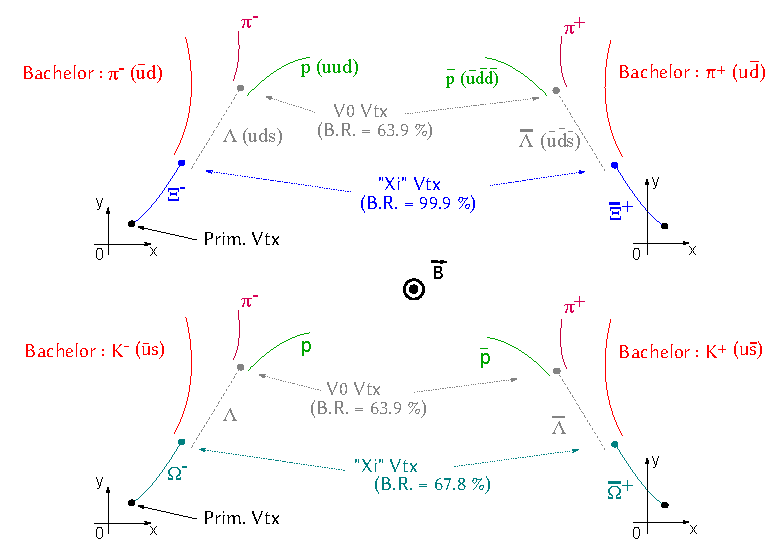
\includegraphics[width=1\textwidth]{Figs/Chapter4/Schema-4TypesDeCascade.eps}
	\caption{Depiction of the full cascade decay chain of the \rmXiM (top left), \rmAxiP (top right), \rmOmegaM (bottom left) and \rmAomegaP (bottom right). Figure taken from \cite{maireFourTypesCascade2011}.}
	\label{fig:CascadeDecay}
\end{figure}

The two decay products continue to travel through the detector, until the baryon daughter decays\footnote{The bachelor daughter being either a \rmPiPlusMinus or \Kplusmin, in most cases it does not decay in the detector due to their long lifetime ($\cTau_{\pi} = 7.8045$ \m and $\cTau_{\rm K} = 3.711$ \m). For those that actually decays in the detector, they are characterised by a \textit{kink} topology due to their decay into a charged particle and a neutral particle.} in  63.9\% of the cases via weak interaction into two oppositely charged particles: a proton and a pion. Depending on their electric charge, one is called the \textit{positive} particle and the other the \textit{negative} particle. This decay topology is known as V0\footnote{The term \say{V0} comes from the V-shape decay topology formed by the two oppositely charged decay daughters.}. Furthermore, the term \say{cascade} refers to the two-steps decay process undergone by the multi-strange baryons. Hence, in the following, the usage of the term \textit{cascade} may be used to mention either the \rmXi or \rmOmega, and similarly the term \textit{V0} for the \rmLambda.

Note that the four cascades on \fig\ref{fig:CascadeDecay} differ only in the nature of the particles involved. On one hand, from the left to right side, the particles are swapped to anti-particles. On the other hand, the larger strangeness content of the \rmOmega imposes the presence of a bachelor particle containing a strange quark (kaon) while, in the \rmXi case, it consists in a light unflavoured meson (pion).

It should also be mentioned that although the \rmXiPM decays into this channel quasi-systematically (99.9\%), this is only the case for 67.8\% of the \rmOmegaPM.\\

\begin{figure}[t]
	\centering
	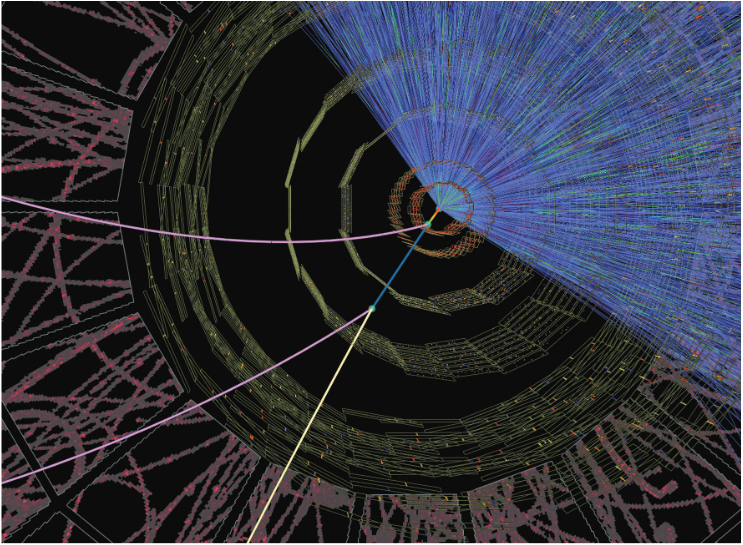
\includegraphics[width=1\textwidth]{Figs/Chapter4/XiEventDisplay.png}
	\caption{Event display of a simulated Pb-Pb collision in the ALICE detector, with a close-up on the ITS. The top part illustrates the typical density of tracks in such environment. The bottom part highlights the cascade decay of a \rmXiM. Figure taken from \cite{alicecollaborationALICEPhysicsPerformance2006}.}
	\label{fig:CascadeDecaySimu}
\end{figure}

\Fig\ref{fig:CascadeDecaySimu} shows the cascade decay of a \rmXiM within the ALICE detector. To make it more apparent, the surrounding tracks have been removed in the bottom left part. The \rmXiPM or \rmOmegaPM being electrically charged, they may loose energy in the detectors and can \textit{a priori} be detected as any other charged particle. Although they can fly over relatively long distance compared to the vast majority of unstable particles, their \cTau remain too short to \textit{systematically} reach the innermost detectors at about 3.9~\cm and 7.6~\cm (to be compared to $\cTau_{\Xi}$ = 4.91 \cm and $\cTau_{\Omega}$ = 2.461 \cm)\footnote{Note that the detection and tracking of these two multi-strange baryons become more likely with the upgraded version of the ITS in the LHC Run-3; the innermost silicon pixel detectors being positioned at a radius of 2.2 \cm and 3.9 \cm in the LHC, the \rmXi and \rmOmega have significantly more chances to leave hits in these detection layers, and therefore to be detected \cite{chinellatoCharmMulticharmBaryon2022}.}. Moreover, the \rmLambda being a neutral particle, it cannot deposit energy in the sensitive layers. In summary, only the bachelor, the positive and negative particles can be detected\footnote{Due to their long lifetime, the detection of the \rmPiPlusMinus, \Kplusmin, \proton and \pbar relies on the reconstruction and identification of their corresponding tracks in the ITS and TPC.}. Therefore, it follows that the V0 and cascade have to be identified indirectly via their decay topology.

The top right part of \fig\ref{fig:CascadeDecaySimu} puts into perspective the difficulty of the reconstructing such a cascade topology in an event with a large combinatorial background. While the bottom part of the figure shows clearly the \rmXiM decay chain, it is actually immersed in a dense environment. In order to identify the multi-strange baryons in the event, the strategy followed in the present work consists in using a topological reconstruction.

\subsection{The principles of the topological reconstruction}
\label{subsec:TopoReco}

The cascade reconstruction is achieved by combining three tracks in the event. The association of two tracks of opposite curvature signs allows to build a \rmLambda (or \rmAlambda) candidate, that may in turn be associated to another track (the bachelor) to form a cascade candidate. In a pp collision, the charged particle density\footnote{per unit of pseudo-rapidity.} can vary from a few particles up to fifty, and more than a thousands in the most central heavy-ion collisions. The mere association of three tracks leads inexorably to the formation of erroneous candidates, thus constituting a source of \textit{combinatorial} background. In order to suppress the latter, geometric selections -- aimed at singling out the candidates spatially compatible with the expected decay topology -- are introduced; this is the general principle behind topological reconstruction.

\subsubsection{Formation of the V0 candidates}
\label{subsubsec:V0Formation}

The reconstruction starts with the formation a V0 candidate. The first step consists in identifying \textit{secondary} tracks, that do not originate from the interaction point. They are tagged as such, if the distance of closest approach (DCA) between the considered track and the primary vertex exceeds a critical value\footnote{While one expects for a primary track to have a DCA to the primary vertex equal (or close) to zero, this is the opposite for a secondary track: since it does not originate from the collision point, its DCA to the interaction vertex must necessarily be different from zero.} (\fig\ref{fig:TopologicalRec}, V0.a). 

The second step aims at forming pairs of secondary tracks of opposite charge, \ie characterised by different curvatures; by imposing that the DCA between the two tracks is small, only the pairs originating potentially from the same decay point are retained. The secondary vertex is then positioned on the segment defined by the previous DCA, weighted by the quality of the tracks (\fig\ref{fig:TopologicalRec}, V0.b).

\afterpage{
\begin{figure}[H]
	\centering
	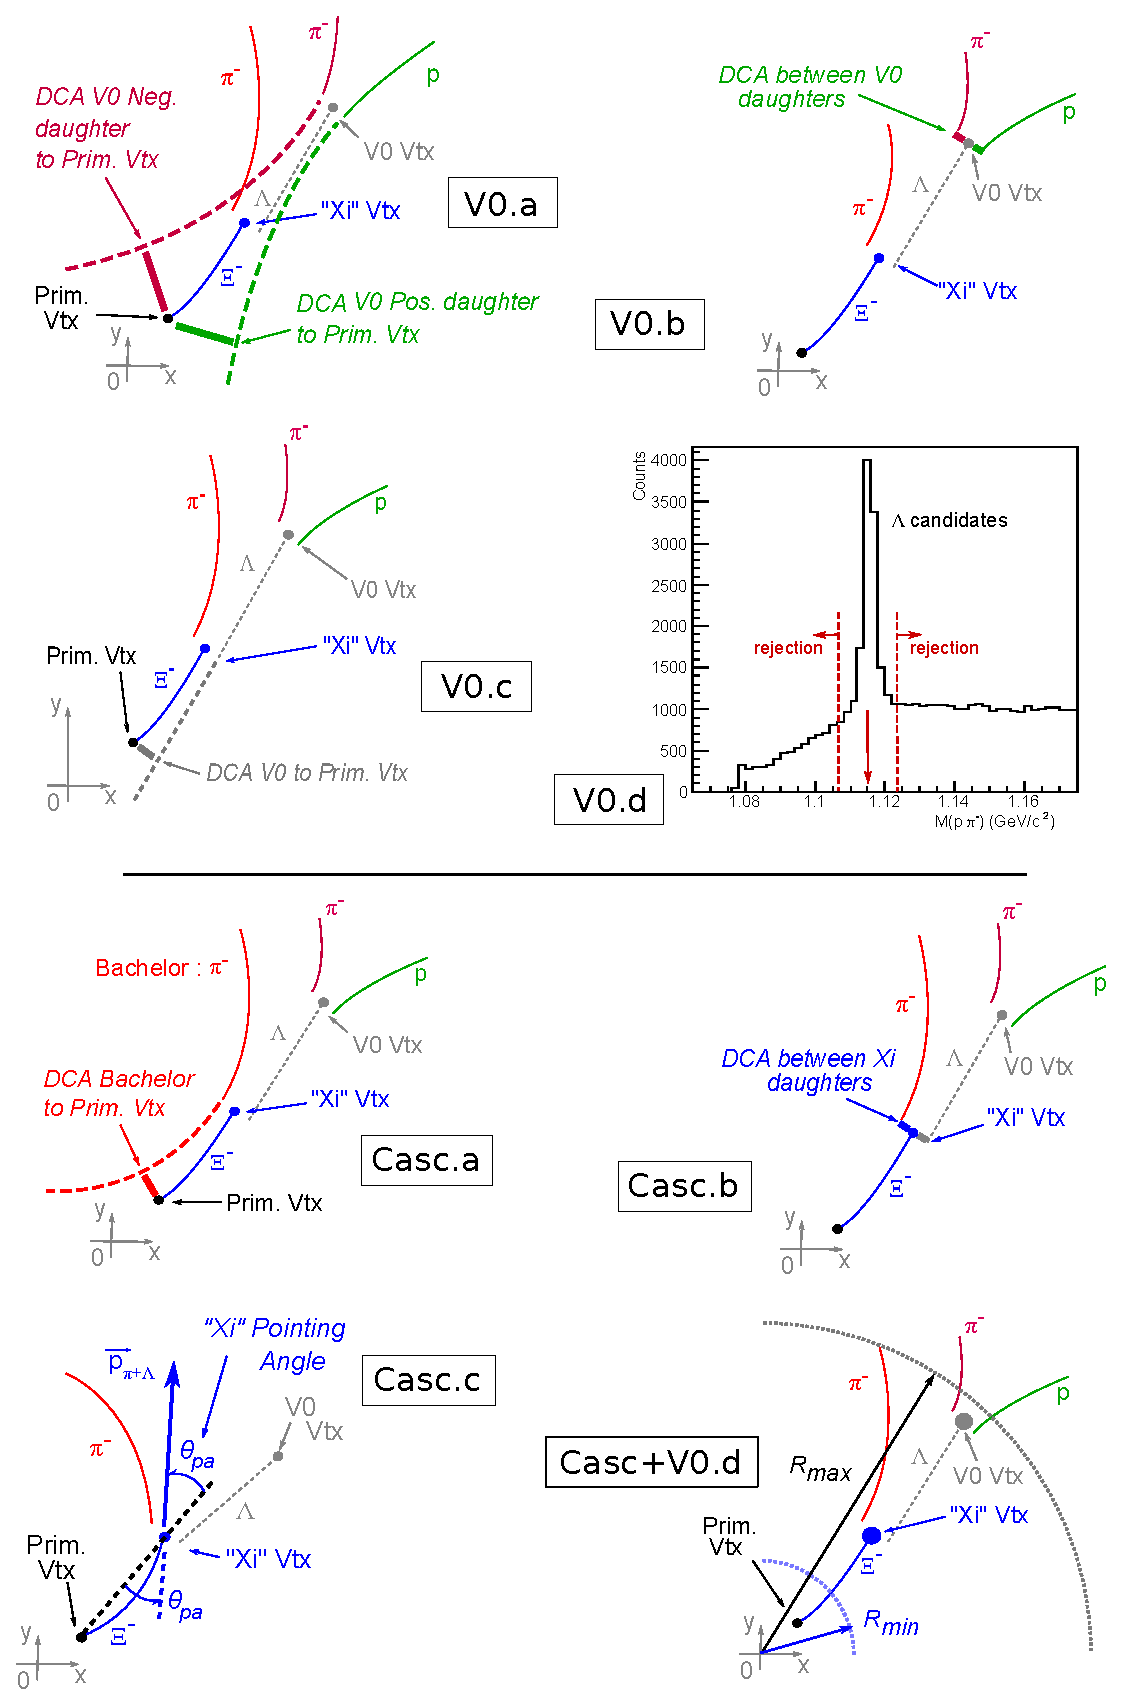
\includegraphics[width=1\textwidth]{Figs/Chapter3/Schema-ExplicationReconstrCascade-en.eps}
	\caption{Schematic representation of the different topological selections applied in order to first reconstruct V0s (top part), and then cascades (bottom part). Figure taken from~\cite{maireTopologicalSelectionsV02011}.}
	\label{fig:TopologicalRec}
\end{figure}
}

The two daughter tracks are then propagated from their initial position (the point of closest approach to the primary vertex, \Sec\ref{subsubsec:TrackReco}) to the secondary decay point\footnote{Most importantly, here the propagation is performed without taking the energy losses into account. This point will be addressed in \chap\ref{chap:CPTAnalysis}\label{footnote:EnergyLossV0CascVertexing}.}. This allows to calculate all the kinematic quantities of the V0, among which its momentum; the latter being equal to the momentum sum of the positive and negative particles at the secondary vertex, due to momentum conservation.

\subsubsection{The reconstruction of cascade candidates}
\label{subsubsec:CascadeFormation}

From the sample of V0 candidates (\Sec\ref{subsubsec:V0Formation}), only those compatible with a \rmXiPM or \rmOmegaPM decay are considered. In other words, the reconstruction of a cascade candidate must necessarily go through a secondary V0 that corresponds to either a \rmLambda or \rmAlambda.\\

Primary and secondary V0s are separated resorting to the pointing direction in the lab frame, given by the momentum at the decay vertex. This direction coincides with the straight-line trajectory of the candidate\footnote{If the candidate corresponds to an actual \rmLambda or \rmAlambda (electrically neutral), its trajectory -- not being curved under the influence of the magnetic field -- must necessarily follow a straight line.} and allows to estimate its DCA to the interaction point (\fig\ref{fig:TopologicalRec}, V0.c). The latter being close to zero for primary V0s, a lower cut on this variable enables their rejection to retain only those tagged as secondary. 

The identification of the V0 goes through the calculation of the invariant mass under  the \rmLambda or \rmAlambda hypothesis. This boils down to making an assumption on the mass of each decay daughter. In the case of a \rmLambda, the positive track corresponds to a proton, the negative to a \piMinus (\eq\ref{eq:LambdaInvMass}); conversely, for a \rmAlambda, they correspond to a \piPlus and an anti-proton respectively. If it turns out that the candidate is, in fact, a true \rmLambda or \rmAlambda, the reconstructed mass should lie within a window of typically a few \mmass\footnote{The width of the mass window depends directly on the ALICE performances in terms of transverse \emph{momentum} resolution, which sits around a few \mmom for low- and intermediate-\pT tracks, that is around a 1\%-level resolution. See \fig\ref{fig:MomResolution} about the track-\pT\ resolution.} (\fig\ref{fig:TopologicalRec}, V0.d), centred around the nominal mass of the \rmLambda,\break $m_{\Lambda} = 1.115683$ \gmass. In most cases, the mis-identification of the daughter particles results in a quite different invariant mass. Therefore, only one of the two mass hypothesis passes the cut, making it possible to differentiate between a \rmLambda and a \rmAlambda.

\begin{align}
M_{\rm candidate}^2(\rmLambda) &= ( E_{\rm pos.} + E_{\rm neg.} )^2 - (\vec{p}_{\rm pos.} + \vec{p}_{\rm neg.})^2 \\
&= \Big(\sqrt{ \vec{p}_{\rm pos.}^2 + m_{\rm pos.}^2} + \sqrt{ \vec{p}_{\rm neg.}^2 + m_{\rm neg.}^2}\Big)^2 - ( \vec{p}_{\rm pos.} + \vec{p}_{\rm neg.})^2\\
&= \Big(\sqrt{ \vec{p}_{\rm pos.}^2 + m_{p^{+}}^2}    + \sqrt{ \vec{p}_{\rm neg.}^2 + m_{\pi^{-}}^2}\Big)^2  - ( \vec{p}_{\rm pos.} + \vec{p}_{\rm neg.})^2 \label{eq:LambdaInvMass}
\end{align}

A last step consists in forming a cascade candidate via the association of a candidate \rmLambda (or \rmAlambda) with any track labelled as secondary\footnote{With the exception of the V0 daughters tracks.} (\fig\ref{fig:TopologicalRec}, Casc.a), playing the role of the bachelor particle. The procedure is analogous to what was done to build a V0 candidate: only pairs with a sufficiently small DCA between the reconstructed \rmLambda (or \rmAlambda) and the bachelor are considered (\fig\ref{fig:TopologicalRec}, Casc.b); primary cascades are set apart from secondary ones by introducing the \textit{pointing angle}. The latter corresponds to the angle defined by the direction of propagation (or pointing direction) of the candidate, and the line joining the primary and secondary vertices. This angle should be small for a primary candidate and, even though the magnetic field is bending their trajectory, the change in direction remains moderate. This selection usually goes through the cosine of the pointing angle, that is constrained to be close to unity in order to validate the cascade as primary (\fig\ref{fig:TopologicalRec}, Casc.c).

The V0 candidate is subject to the same cut. Due to its large mass compared to the one of the bachelor, the reconstructed \rmLambda (or \rmAlambda) takes up most of the cascade momentum, and so most of the pointing direction. As a consequence, in order to ensure that the V0 actually originates from a \rmXiPM or \rmOmegaPM decay, the cosine of its pointing angle has to be close to unity.\\

As a final topological selection, the cascade and V0 decay vertices must lie within a certain confidence area, in the transverse plane (\fig\ref{fig:TopologicalRec}, Casc.d). Close to the interaction point, at small radii, the combinatorial background is overwhelming due to the high density of tracks. Conversely, at large distance, the probability of finding a \rmXiPM or \rmOmegaPM becomes extremely low. For comparison, the inner wall of the TPC ($\sim$ 85 \cm) lie at $\sim 18$ $\cTau_{\Xi}$ and $\sim 35$ $\cTau_{\Omega}$. At such distance, the \rmXiPM and \rmOmegaPM survival probabilities are about 2\% and 0.001\%\footnote{Considering a high-momentum cascade of 5 \gmom.} respectively. Therefore, the decay vertices of both cascade and V0 must be located beyond a radius deemed critical; those decaying too far away with respect to their lifetime are rejected\footnote{Note that one consists in a selection on the \emph{radial} position of the decay vertices, the other, in a cut on their \emph{3D} location.}.

\subsubsection{Invariant mass of the cascade candidates}
\label{subsubsec:InvariantMassSelection}

At this stage, the topological reconstruction is over; each triplet of tracks forms a cascade candidate, that can correspond to a \rmXiPM, a \rmOmegaPM or some residual background. The distinction is made based on the invariant mass of each candidate (\eq\ref{eq:CascInvMass}).

\begin{align}
M_{\rm candidate}^2( \textrm{casc.}) &= ( E_{\rm V0} + E_{\rm bach.} )^2 - ( \vec{p}_{\rm V0} + \vec{p}_{\rm bach.})^2 \\
&= \Big(\sqrt{ \vec{p}_{\rm V0}^2 + m_{\rmLambda}^2} + \sqrt{ \vec{p}_{\rm bach.}^2 + m_{\rm bach.}^2}\Big)^2 - ( \vec{p}_{\rm V0} + \vec{p}_{\rm bach.})^2 \label{eq:CascInvMass}
\end{align}

\begin{align}
M_{\rm candidate}^2( \rmXiPM ) &= \Big(\sqrt{ \vec{p}_{\rm V0}^2 + m_{\rmLambdaPM}^2} + \sqrt{ \vec{p}_{\rm bach.}^2 + m_{\pi^{\pm}}^2}\Big)^2 - ( \vec{p}_{\rm V0} + \vec{p}_{\rm bach.})^2 \label{eq:XiInvMass} \\
M_{\rm candidate}^2( \rmOmegaPM ) &= \Big(\sqrt{ \vec{p}_{\rm V0}^2 + m_{\rmLambdaPM}^2} + \sqrt{ \vec{p}_{\rm bach.}^2 + m_{\rm K^{\pm}}^2}\Big)^2 - ( \vec{p}_{\rm V0} + \vec{p}_{\rm bach.})^2
\label{eq:OmegaInvMass}
\end{align}

For each association of three particles (\ie one cascade candidate), two invariant masses are calculated: one under the hypothesis of a \rmXiPM candidate (\eq\ref{eq:XiInvMass}), the other for a \rmOmegaPM candidate (\eq\ref{eq:OmegaInvMass}). Note that, contrarily to the \rmLambda and \rmAlambda cases, the numeric value of the invariant mass is the same for the \say{particle} (\rmXiM, \rmOmegaM) and the \say{anti-particle} calculations (\rmAxiP, \rmAomegaP). The mass roles do not swap among the two decay daughters, V0 and bachelor; only the sign of the bachelor's electric charge allows to distinguish between particle and anti-particle. In addition, the masses of the daughter particles involved in \eq\ref{eq:XiInvMass} and \ref{eq:OmegaInvMass} correspond, in fact, to the nominal values from the PDG \cite{particledatagroupReviewParticlePhysics2022}; most importantly, that means that the reconstructed mass of the V0 is not being used here, \ie the PDG mass \mPDG[\rmLambda] is used instead. As long as the latter has been identified as a \rmLambdaPM (\ie its mass fits into a certain tolerance window, \Sec\ref{subsubsec:CascadeFormation}), this choice has the advantage of limiting the deterioration on the cascade invariant mass resolution. \\

Although the invariant mass allows to distinguish a \rmXiPM from a \rmOmegaPM, there exists a region where this is not possible anymore. \Fig\ref{fig:MassXiVsOmega} shows the invariant mass distribution of cascade candidates assuming a \rmOmegaM as a function of the same candidate under the hypothesis of a \rmXiM. There are two discernible and perpendicular mass bands, each one corresponding to the true population of one of two considered species. At their intersection, the two species become indistinguishables -- they compete, in some sense -- which results in an increased background in this region: a candidate identified as \rmXiM may, in fact, reveal to be a \rmOmegaM, and vice-versa.

This additional background affects each kind of cascade in different proportions, though. Since the population of true \rmXiM is much larger than the one of \mbox{\rmOmegaM\footnote{That is because the \rmXi are typically ten times more produced than the \rmOmega~\cite{alicecollaborationProductionLightflavorHadrons2021}.}}, the latter constitutes a marginal source of background with respect to the \rmXiM. Conversely, the true \rmXiM hyperons -- particularly in the low mass region -- represent a considerable source of background for the \rmOmegaM. As a consequence, in the context of the reconstruction of \rmOmegaPM baryons, any candidates also identified as a \rmXiPM\ -- that is, with an invariant mass under the assumption of a \rmXiPM within a window of few~\mmass around \mPDG[\rmXi]\ -- are rejected.

\begin{figure}[!t]
	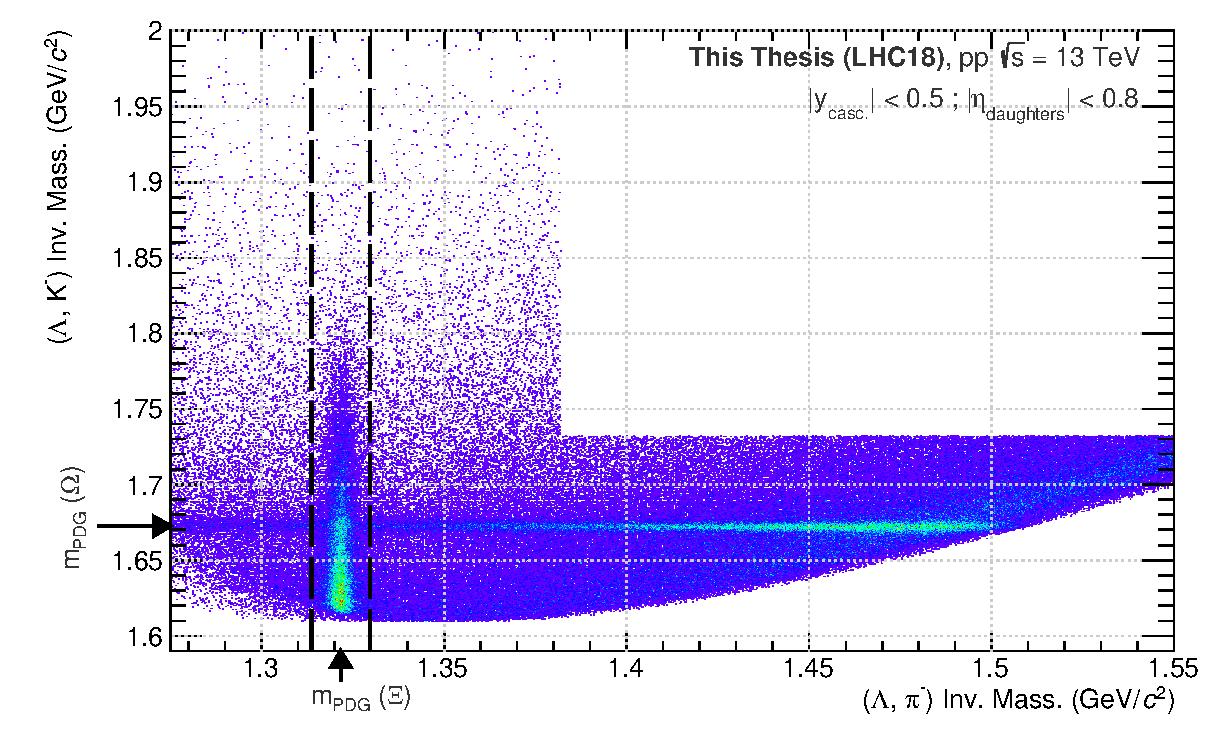
\includegraphics[width=0.9\textwidth]{Figs/Chapter4/MassXiVsOmegaMinus.eps}
	\caption{Invariant mass distribution under the \rmOmegaM and \rmXiM mass hypotheses, each cascade candidate can be seen under one hypothesis or the other (\eq\ref{eq:XiInvMass} and \ref{eq:OmegaInvMass}). The dashed lines show the mass rejection $\mPDG[\rmXi] \pm 0.008~\gmass$, applied in the reconstruction of a \rmOmegaPM candidate.}
	\label{fig:MassXiVsOmega}
\end{figure}



\subsection{The context of hyperon reconstruction in ALICE}
\label{subsec:HyperonAndALICE}

In view of their characteristics, the reconstruction of multi-strange baryons requires excellent detection capabilities. In that regard, few experiments can compete with the performances of the ALICE detector at mid-rapidity.

As already outlined in \Sec\ref{subsec:ALICEDetector}, the high granularity of its inner tracker allows to reconstruct the primary vertex, as well as the secondary vertices from V0 and cascade decays, with a precision better than 100 \mum\footnote{Not to mention the resolution on the DCA of the daughter tracks to the primary vertex of about 30 \mum \cite{alicecollaborationPerformanceALICEExperiment2014}.}. Thanks to its large lever arm and almost continuous sampling of the particle trajectory, the TPC 
provides an excellent momentum measurement with a resolution of 0.7\%\footnote{This obviously depends on the track momentum; here this is for \pT = 1 \gmom.} \cite{alicecollaborationALICEPhysicsPerformance2006}, as well as a robust particle identification. Hence, the TPC ensures an efficient reconstruction and identification of the hyperon's decay daughters, and thus of the hyperon itself. Coupled with its extremely low material budget (13\% \Xzero\ up to the outer wall of the TPC) and moderate magnetic field of 0.5 T, the strange hadron reconstruction can be performed over a wide momentum range and particularly, at low \pT, where the most important part of the production is.

Furthermore, the experiment benefits from the high-energy collisions delivered by the LHC. At such energies, matter and anti-matter are produced in almost equal proportions, offering the opportunity to study simultaneously hyperons and anti-hyperons. For all these reasons, ALICE stands as a perfectly suited experiment to analyse multi-strange baryons. \\

It should be emphasized that the cascade reconstruction varies with the track density, that goes from a few charged particles in pp collisions up to 2000 at mid-rapidity in the most central Pb-Pb collisions at \sqrtSnn = 5.02 \tev \cite{alicecollaborationCentralityDependenceChargedParticle2016}. In heavy-ion collisions, the enormous amount of tracks means a larger background, but also a larger number of contributor for the primary vertex determination and hence a better resolution on its position. This is in contrast with the pp environment, where the events are less dense but the quality of the primary vertex reconstruction is poorer. Therefore, the topological selections shall be adapted for each environment, as these differences may lead to various biases on the DCA to the primary vertex, pointing angles, etc.

Also, a compromise has to be found between purity and reconstruction efficiency. In both cases, the key point revolves around the treatement of the background, which depends on the physics analysis. For example, if the background -- or more precisely, its shape -- is known in advance, the latter becomes tolerable as it can be subtracted later; thus, one may favour a high efficiency (\ie relatively loose selections). In the reverse situation  where the background is unknown, it seems preferable to apply tighter cuts in order to keep a signal with a low level of contamination, thus ensuring a high signal purity.

